\documentclass[UTF8]{ctexart}

\usepackage{subfiles}  

%下面的语句, 引入你的头部设置文件
\usepackage{C:/phpStorm_proj/02_myself_ID_EGO/+100_latex_all_math_sel/myPreamble} 
%必须是绝对路径,才能让各个tex在单独编译时使用到

\title{导数 Derivative}




%------------------------------------------------------------



\begin{document}
	\tableofcontents % 生成目录
	\date{} % 若不写这句, 则默认也会渲染出日期, 所以我们要手动赋空值	
	\maketitle  %这行代码, 让你前面的 title, author, date生效




\part{什么是导数?}

某点处的``导数", 就是该点处``切线的斜率".

导数, 就是一个``极限值", 比如, y 在 点$x_0$ 处的导数, 就是:  $f'(x_0) = \lim_{\Delta x \to 0} \dfrac{\Delta y} {\Delta x} $


\begin{figure}[htbp]%调节图片位置,h:浮动;t:顶部;b:底部;p:当前位置
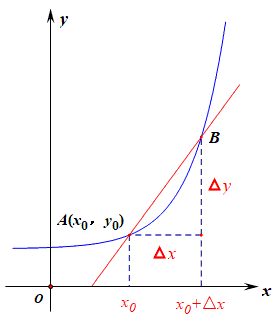
\includegraphics[width=0.25\textwidth]{/0023.png}
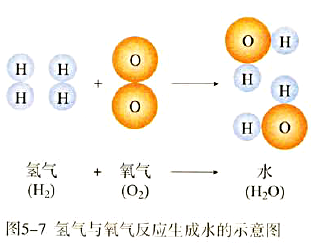
\includegraphics[width=0.25\textwidth]{/0024.png}
\end{figure}


可导, 就意味着图像很"光滑". 即图像没有"尖角"存在 (因为尖角处的左右导数不相等).

并且, 切线不能垂直于x轴. 如果切线是垂直于x轴的, 它的斜率就会是 +∞ 或 -∞了. \\



$x_0$ 点处的导数, 其实可以有下面4种写法来表示: 

(1) $y'|_{x=x_0}$

(2)  $f'(x_0)$

(3)  $\dfrac{dy} {dx}|_{x=x_0}$

(4) $\dfrac{d f(x)} {dx}|_{x=x_0}$ \\


``位置"的瞬时变化率(变换趋势, 能预测未来), 就是``速度". 所以速度是位置的导数. 

``速度"的瞬时变化率, 就是``加速度". 所以``加速度"是``速度"的导数. ``加速度"就是``位置"的二阶导.  \\

单侧导数, 就是从``某一侧"逼近某一x点时, 该点的切斜斜率.

所以, 左导数, 就是``从左侧向右"逼近了. 右导数, 就是``从右边向左"逼近了.

- 左导数 : $f_{-}^{’}\left( x_0 \right) =\lim_{x\rightarrow x_{0}^{-}}\dfrac{f\left( x \right) -f\left( x_0 \right)}{x-x_0}\\ $
- 右导数 : $f_{+}^{’}\left( x_0 \right) =\lim_{x\rightarrow x_{0}^{+}}\dfrac{f\left( x \right) -f\left( x_0 \right)}{x-x_0}\\ $


~\\
\hrule
~\\


\part{导数公式}

\section{常用的导数}



\subsection{$(\text{常数}C)' =0$}

常数不会变化, 自然没有``瞬时变化率"存在, 所以常数的导数就=0.





\subsection{$(x^n)'= n x^{n-1}$}

(1) 当指数 n=1时, 其导数=1. 

(2)  当 $n \textgreater 1$ 时, 其导数是 $ (x^n)' = n x^{n-1}$ \\

\begin{myEnvSample}
求 $ y= \dfrac{1} {x}$  在 点(1/2, 2)处的切线的斜率(即导数), 并求出该切线的方程.

其导数是: $y'=\left( x^{-1} \right) '=-1x^{-1-1}=-1x^{-2}$

然后把 点(x=1/2, y=2) 代入进去, 得到: $y'\mid_{x=\frac{1}{2}}^{}=-1\left( \frac{1}{2} \right) ^{-2}=-4$  ← 这个数值, 就是 函数在点(1/2, 2)处的切线的斜率.

然后再套用直线的``点斜式方程" $y - y_1 = k(x- x_1)$

本例的切线即: $y-\underset{=2}{\underbrace{y_1}}=\underset{\text{即}y'=-4}{\underbrace{k}}\left( x-\underset{=\frac{1}{2}}{\underbrace{x_1}} \right)$
\end{myEnvSample}





\subsection{$\left( a^x \right) '=a^x\ln a$}

即直接后面跟个尾巴: ln a

例如, $(2^x)' = 2^x \ln 2$




\subsection{$(e^x)' = e^x \ln e = e^x$}

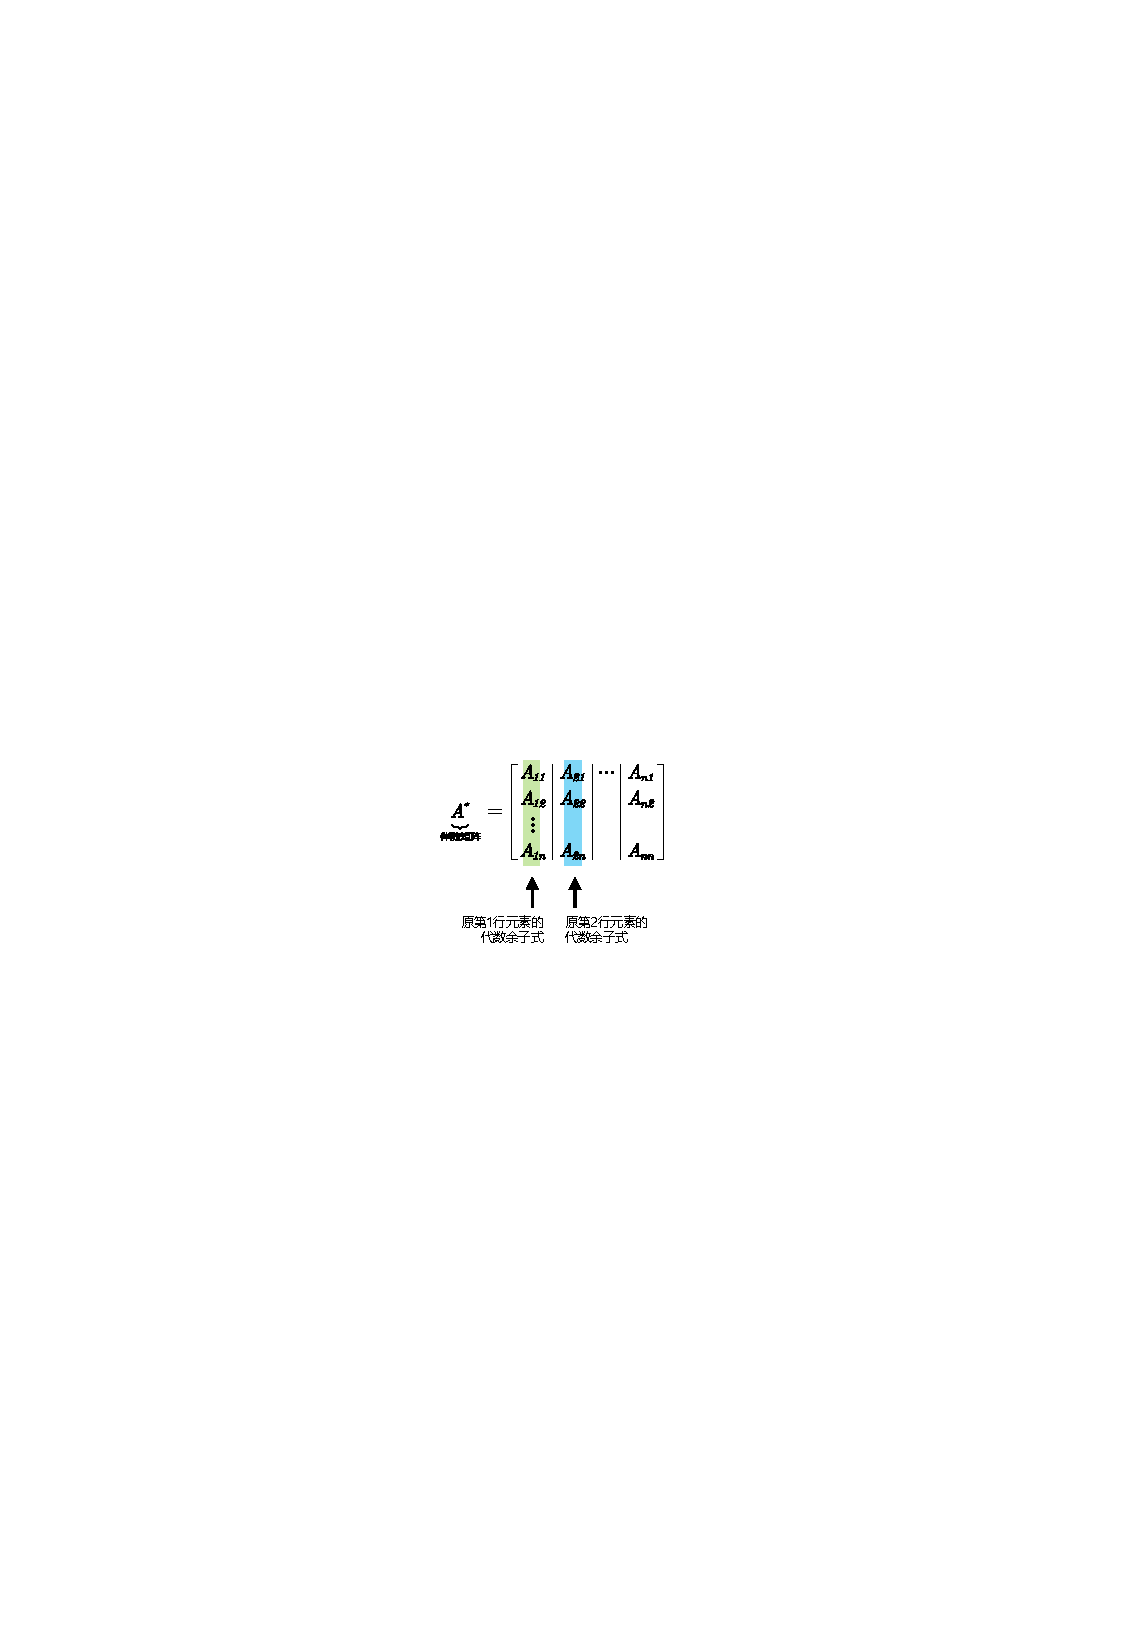
\includegraphics[width=0.5\textwidth]{/0025.pdf}




\subsection{$(\log_a x)' = \dfrac{1} {x \ln a}$}

即把 x 提到前面去, 把log 变成 ln, 整体再放在分母上. 分子为1. \\

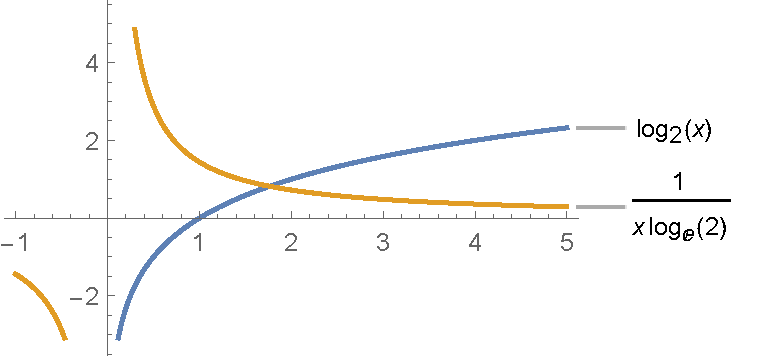
\includegraphics[width=0.5\textwidth]{/0026.pdf}



\subsection{$(\ln x)' = \dfrac{1} {x}$}

例如: 
$\left( \log _ex \right) '=\dfrac{1}{x\underset{=\log _ee=1}{\underbrace{\ln e}}}=\dfrac{1}{x}$ \\


\textbf{对``对数函数"求导, 有一种技巧: 换底成ln后再来做. 因为转成ln后, 操作会变得简单.} \\

\begin{myEnvSample}
	\begin{align*}
	&y=x^x,\ \text{求}y'\\
&\ln\text{(}y\text{)}=\ln\text{(}x^x\text{)\ }\gets \text{两边同时取}\ln\\
&\ln\text{(}y\text{)}=x\ln x\\
&\left( \ln y \right) '=\left( x\ln x \right) '\ \gets \text{两边同时对}x\text{求导,注意}y\text{是个复合函数,要用剥洋葱法}\\
&\ln\text{'}y\cdot y'=x'\ln x+x\text{(}\ln x\text{)'}\\
&\frac{1}{y}\cdot y'=1\cdot \ln x+x\frac{1}{x}\\
&y'=\left( \ln x+1 \right) y\ \gets \text{再把}y\text{这个复合函数的具体内容}=x^x\text{代进去}\\
&y'=\left( \ln x+1 \right) x^x
	\end{align*}
\end{myEnvSample}





\section{反函数的导数 : $\boxed{[f^{-1}(y)]' = \dfrac{1} {\text{原函数的导数} f'(x)}}$}


反函数的导数, 和其原函数的导数, 呈``倒数关系". 

原函数是 y=f(x), 其反函数是 x=f(y), 则, 反函数的导数, 就是``原函数导数"的倒数. 


换言之, 原函数的导数是 $\dfrac{\varDelta y}{\varDelta x} $, , 则其反函数的导数就是  $\dfrac{1}{\frac{\varDelta y}{\varDelta x}}$.

\textbf{``原函数"和``反函数", 它们``导数"的乘积 =1.}

``原函数"与其``反函数"的图像, 是关于 y=x 对称的.




\section{三角函数的导数}

\subsection{$(\sin x)' = \cos x$}

\subsection{$(\cos x)' = -\sin x$}

\subsection{$(\tan x)' = \sec^2 x$}

\subsection{$(\cot x)' = -\csc^2 x$}

\subsection{$(\sec x)' = \sec x  \cdot \tan x$}

\subsection{ $(\csc x)' = - \csc x \cdot \cot x$}





\section{反三角函数的导数}

\subsection{$(\arcsin x)' = \dfrac{1} {\sqrt{1-x^2}}$}

\subsection{$(\arccos x)' = - \dfrac{1} {\sqrt{1-x^2}}$}

\subsection{$(\arctan x)' =  \dfrac{1} {1 + x^2}$}

\subsection{$(\operatorname{arccot}  x)' = - \dfrac{1} {1 + x^2}$}


~\\
\hrule
~\\



\part{求导的各种方法, 方法论}



\section{求导法则 : 和差积商}


\subsection{$(a+b)' = a'+b'$}

例: $ \left( x^2+\sin x \right) '=\left( x^2 \right) '+\left( \sin x \right) '=2x +\cos x $


\subsection{$(a+b)' = a'+b'$}

\subsection{$(a+b+c)' = a'+b'+c'$}

\subsection{$(a-b)' = a' - b'$}

\subsection{$(ab)' = a'b + ab'$}
例: $(x^3 e^x)'=(x^3)' e^x + x^3 (e^x)' = 3x^2 e^x + x_3 e^x$


\subsection{$(abc)' = a'bc + ab'c + abc'$}


\subsection{$(\text{常数C} \cdot a)' = C \cdot a'$} ← 直接把常数提到外面去就行了

例: $(5 sinx)'=5(sinx)'=5 cosx$


\subsection{$(\dfrac{a} {b})' = \dfrac{a'b - ab'} {b^2}$}
即: $\left( \frac{\text{上}}{\text{下}} \right) '=\dfrac{\text{上'}\cdot \text{下}-\text{上}\cdot \text{下'}}{\text{下}^2}$




\section{对``复合函数"求导的方法: 链式法则 / 剥洋葱法}

\begin{align*}  % 支持每行编号. 若不需要编号, 就用 align*环境
\text{有}\left\{ \begin{array}{l}
	\text{大}=f\text{(中)}\\
	\text{中}=g\text{(小)}\\
	\text{小}=h\text{(微)}\\
\end{array},\ \ \text{则:}\frac{d\text{大}}{d\text{微}}=\frac{d\text{大}}{d\text{中}}\cdot \frac{d\text{中}}{d\text{小}}\cdot \frac{d\text{小}}{d\text{微}} \right. 
\end{align*}


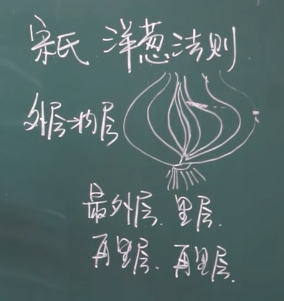
\includegraphics[width=0.2\textwidth]{/0027.png} \\


\begin{myEnvSample}
	我们用``剥洋葱法"(从外向内一层层求导), 来求下面的复合函数 的导数
	\begin{align*}
		& y=\left( 1-2x^2 \right) ^{\frac{1}{3}} \\
		& y'=\left[ \left( 1-2x^2 \right) ^{\frac{1}{3}} \right] '\cdot \left( 1-2x^2 \right) '=\frac{1}{3}\left( 1-2x^2 \right) ^{\frac{1}{3}-1}\cdot \left( -2\cdot 2x \right) 		
	\end{align*}
\end{myEnvSample}




\section{对``参数方程"求导的方法}

比如, 有这个参数方程, t是参数 : 
\[ d(x)=
\begin{cases}
	x= f(t) \\
	y= g(t)
\end{cases}
\]

要求``y对x求导". 则:

其``一阶导数"是: $\dfrac{dy}{dx}=\dfrac{g'\text{(}t\text{)}}{f'\text{(}t\text{)}}=\dfrac{y\text{对}t\text{的导数}}{x\text{对}t\text{的导数}}=\dfrac{\dfrac{dy}{dt}}{\dfrac{dx}{dt}} $


其``二阶导数"是: $ \dfrac{d^2\text{(}y\text{)}}{dx^2}=\dfrac{d}{dx}\left( \dfrac{dy}{dx} \right) =\dfrac{\dfrac{dy}{dx}\text{对}t\text{的导数}}{x\text{对}t\text{的导数}}=\dfrac{\dfrac{d}{dt}\left( \dfrac{dy}{dx} \right)}{\dfrac{dx}{dt}} $




\section{对``隐函数"求导的方法}

- 显函数: 能清晰的写成 y= ...x 的形式.

- 而隐函数: 虽然 x和y之间有关系, 但无法写成清晰的 $ y=f(x)$ 的形式. 即无法变换成``能把y单独提取出来, 放在等号左边"的这种形式. \\

\textbf{对``隐函数"求导的方法是: 等号两边同时对 x 求导.} \\

\begin{myEnvSample}
	\begin{align*}
	&\text{有隐函数\ }e^y+xy-e=0,\text{求}y'\\
&\text{(}e^y+xy-e\text{)'}=0'\\
&\text{(}e^y\text{)'}y'+\text{(}xy\text{)'}-e'=0\ \gets \text{常数}e\text{的导数也}=0\\
&e^yy'+\text{(}x'y+xy'\text{)}=0\\
&e^yy'+y+xy'=0\\
&\text{(}e^y+x\text{)}y'=-y\\
&y'=-\frac{y}{\text{(}e^y+x\text{)}}
	\end{align*} 

因为是隐函数, y 无法写成 ...x的形式, 所以我们就会发现, y'的结果里面, 也无法只有纯粹的x, 会带着y.
\end{myEnvSample} 



\begin{myEnvSample}
	\begin{align*}
		&y=e^xx^2\ln x\tan x\ \gets \text{先两边取}\ln\text{,转成对数}\\
	&\ln y=\ln \left( e^xx^2\ln x\tan x \right) \ \gets \text{根据公式}\ln \left( ab \right) =\ln a+\ln b\\
	&\ln y=\ln e^x+\ln x^2+\ln \left( \ln x \right) +\ln \left( \tan x \right) \ \gets \text{再两边求导}\\
	&\left( \ln y \right) '\cdot y'=\underset{\begin{matrix}
			=\left( x\ln e \right) '\\
			=\left( x\cdot 1 \right) '\\
			=1\\
	&\end{matrix}}{\underbrace{\left( \ln e^x \right) '}}+\underset{\begin{matrix}
			=\frac{1}{x^2}2x\\
			=\frac{2}{x}\\
	&\end{matrix}}{\underbrace{\left( \ln x^2 \right) '}}+\underset{=\frac{1}{\ln x}\frac{1}{x}}{\underbrace{\left( \ln \left( \ln x \right) \right) '}}+\underset{\frac{1}{\tan x}\sec ^2x}{\underbrace{\left( \ln \left( \tan x \right) \right) '}}\\
	&\frac{1}{y}y'=\frac{2}{x}+\frac{1}{x\ln x}+\frac{\sec ^2x}{\tan x}\\
	&y'=\left( \frac{2}{x}+\frac{1}{x\ln x}+\frac{\sec ^2x}{\tan x} \right) y\ \gets \text{然后把}y\text{的具体值}=e^x\cdot x^2\cdot \ln x\cdot \tan x\text{代入进去}\\
	&y'=\left( \frac{2}{x}+\frac{1}{x\ln x}+\frac{\sec ^2x}{\tan x} \right) \left( e^x\cdot x^2\cdot \ln x\cdot \tan x \right)	
	\end{align*}
\end{myEnvSample}





\end{document}

